\section{Numerical Results}
\label{sec:results}

To test and verify the implementation of the \gls{qahps} method, we solve two Poisson equations and one Helmholtz equation. For each, we present error, timing, and memory usage results and discuss the performance of our implemented method.

For all of our examples, we discretize the Laplace operator at the patch level using a second-order, 5-point stencil on a finite volume (cell-centered) mesh. The code is implemented as part of EllipticForest \citep{chipman2024ellipticforest}. EllipticForest is written primarily in C++, with wrappers to FORTRAN routines to call FISHPACK and LAPACK \citep{anderson1999lapack} for any dense linear algebra operations (more on EllipticForest in \refsec{sub:elliptic-forest}). The mesh and solution are output into an unstructured VTK mesh file \citep{kitware2006vtkBook} and are visualized with the VisIt software \citep{HPV:VisIt}. All tests were run on a 2021 MacBook Pro with an M1 Pro CPU and 32 GB of RAM.

\subsection{Poisson Equation 1}
\label{sub:example_one}

We solve the following boundary value problem:
\begin{align}
    \nabla^2 u(x,y) = -(\sin(x) + \sin(y))
\end{align}
on the square domain $\Omega = [-10, 10] \times [-10, 10]$, subject to Dirichlet boundary conditions $u(x,y) = g(x,y)$ on the boundary which is computed according to the exact solution
\begin{align}
    u_{exact}(x,y) &= \sin(x) + \sin(y).
\end{align}

For the refinement criteria, we refine according to the right-hand side function $f(x,y)$, which corresponds to the curvature of the solution. We set a refinement threshold of $1.2$ and refine a patch when $f(x,y) > 1.2$ for any $x,y$ in a patch. This results in a mesh and solution that can be found in \reffig{fig:poisson_plot}.

\begin{figure}
    \centering
    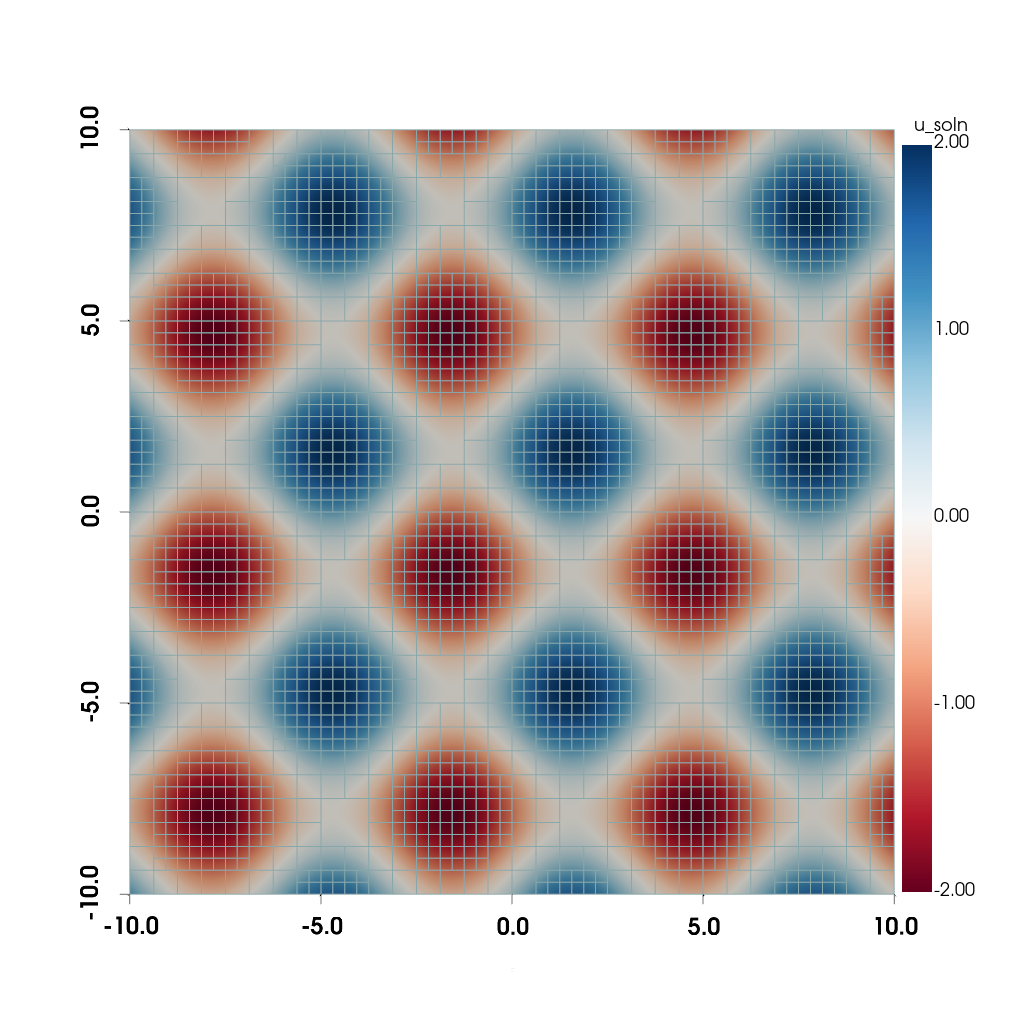
\includegraphics[width=0.75\textwidth, trim={0 100 0 0}]{figures/plot_poisson.png}
    \caption{The computed solution and mesh for the Poisson problem from \refsec{sub:example_one}.  Patch size for this plot is $16 \times 16$ and mesh is refined to level 7.  Refinement criteria is based on the magnitude of the right hand side function $f(x,y)$.}
    \label{fig:poisson_plot}
\end{figure}

{\bf Results and Discussion}
Tables \ref{tab:poisson_error} and \ref{tab:poisson_timing} show the error, timing, and memory results for the current implementation on this Poisson equation. \reftab{tab:poisson_error} shows results for both a uniformly refined mesh (a mesh without any coarse-fine interfaces or local adaptivity) and results for the adaptive mesh case. For the uniform case, we get the expected second order convergence in both the $L_{\infty}$ and $L_1$ norms. The adaptive case mostly shows second order convergence, except for a few cases where the refinement between successive levels results in a smaller jump in error than second order provides. \reftab{tab:poisson_timing} shows timing and memory results for the same case. Here, the difference between the uniform and adaptive case is highlighted. The adaptive case gives a $4.5$ times speed up for the build stage, and nearly a $20$ times speed up for the solve stage. Memory used to store the quadtree and operators is also significantly reduced with the adaptive case.

\begin{table}
    \caption{Convergence analysis for the Poisson equation (\refsec{sub:example_one}). The upper part shows convergence for a uniformly refined mesh, while the lower part shows convergence for an adaptively refined mesh. $M$ is the size of the grid on each leaf patch, $L_{\text{max}}$ is the maximum level of refinement, $R_{\text{eff}}$ is the effective resolution for a uniformly refined mesh, DOFs is the total degrees of freedom (i.e., total mesh points), $L_{\infty}$ error is the infinity norm error, $L_{\infty}$ order is the infinity norm convergence order, $L_1$ error is the $1^{\text{st}}$ norm error, and $L_1$ order is the $1^{\text{st}}$ norm convergence order.}
    \centering
    \sisetup{
        table-alignment-mode=format
    }
    \begin{tabular}{
        |
        S   % Patch size
        S[table-column-width=0.8cm]   % Max level
        S[table-text-alignment=right, table-column-width=0.7cm]   % Effective resolution
        S[table-text-alignment=right, table-column-width=1.4cm]   % DOFs
        S[scientific-notation=true, round-mode=places, round-precision=2, table-column-width=1.65cm]   % L-inf error
        S[scientific-notation=false, exponent-mode=fixed, round-mode=places, round-precision=2, table-column-width=1.5cm]   % L-inf order
        S[scientific-notation=true, round-mode=places, round-precision=2]   % L-1 error
        S[scientific-notation=false, exponent-mode=fixed, round-mode=places, round-precision=2]   % L-1 order
        |
    }
\hline
{M} & {$L_{\text{max}}$} & {$R_{\text{eff}}$} & {DOFs} & {$L_{\infty}$ Error} & {$L_{\infty}$ Order} & {$L_1$ Error} & {$L_1$ Order} \\
\hline
% \num{16} & \num{1} & \num{32} & \num{1024} & \num{7.2721827038740E-02} & {--} & \num{2.3319531214882E-02} & {--} \\
% \num{16} & \num{2} & \num{64} & \num{4096} & \num{1.7803276283615E-02} & \num{2.0302456853013E+00} & \num{5.7570511934287E-03} & \num{2.0181368404886E+00} \\
% \num{16} & \num{3} & \num{128} & \num{16384} & \num{4.4594278588197E-03} & \num{1.9972122300096E+00} & \num{1.4365857848192E-03} & \num{2.0026858961169E+00} \\
\num{16} & \num{4} & \num{256} & \num{65536} & \num{1.1146466297640E-03} & \num{2.0002722123237E+00} & \num{3.5892082197986E-04} & \num{2.0009066196875E+00} \\
\num{16} & \num{5} & \num{512} & \num{262144} & \num{2.7855514231123E-04} & \num{2.0005515585727E+00} & \num{8.9717104596707E-05} & \num{2.0002106534890E+00} \\
\num{16} & \num{6} & \num{1024} & \num{1048576} & \num{6.9642847198903E-05} & \num{1.9999158585307E+00} & \num{2.2428541266291E-05} & \num{2.0000472698832E+00} \\
\num{16} & \num{7} & \num{2048} & \num{4194304} & \num{1.7410906046011E-05} & \num{1.9999839043577E+00} & \num{5.6070914295010E-06} & \num{2.0000112920243E+00} \\
% \num{32} & \num{1} & \num{64} & \num{4096} & \num{1.7803276283615E-02} & {--} & \num{5.7570511934284E-03} & {--} \\
% \num{32} & \num{2} & \num{128} & \num{16384} & \num{4.4594278588175E-03} & \num{1.9972122300103E+00} & \num{1.4365857848190E-03} & \num{2.0026858961170E+00} \\
% \num{32} & \num{3} & \num{256} & \num{65536} & \num{1.1146466297716E-03} & \num{2.0002722123132E+00} & \num{3.5892082198209E-04} & \num{2.0009066196784E+00} \\
\num{32} & \num{4} & \num{512} & \num{262144} & \num{2.7855514234232E-04} & \num{2.0005515584215E+00} & \num{8.9717104608167E-05} & \num{2.0002106533137E+00} \\
\num{32} & \num{5} & \num{1024} & \num{1048576} & \num{6.9642847325024E-05} & \num{1.9999158560790E+00} & \num{2.2428541313515E-05} & \num{2.0000472670298E+00} \\
\num{32} & \num{6} & \num{2048} & \num{4194304} & \num{1.7410906499649E-05} & \num{1.9999838693813E+00} & \num{5.6070916187308E-06} & \num{2.0000112463735E+00} \\
\hline
% \num{16} & \num{1} & \num{32} & \num{1024} & \num{7.2721827038740E-02} & {--} & \num{2.3319531214882E-02} & {--} \\
% \num{16} & \num{2} & \num{64} & \num{4096} & \num{1.7803276283615E-02} & \num{2.0302456853013E+00} & \num{5.7570511934287E-03} & \num{2.0181368404886E+00} \\
% \num{16} & \num{3} & \num{128} & \num{16384} & \num{4.4594278588197E-03} & \num{1.9972122300096E+00} & \num{1.4365857848192E-03} & \num{2.0026858961169E+00} \\
\num{16} & \num{4} & \num{256} & \num{64000} & \num{2.5910957992683E-03} & \num{7.8329626881446E-01} & \num{4.4586170147130E-04} & \num{1.6879759592817E+00} \\
\num{16} & \num{5} & \num{512} & \num{194560} & \num{6.6263501289099E-04} & \num{1.9672760156010E+00} & \num{1.2477150864153E-04} & \num{1.8373077457909E+00} \\
\num{16} & \num{6} & \num{1024} & \num{569344} & \num{6.8094879278413E-04} & \num{-3.9331876110758E-02} & \num{1.0216613949030E-04} & \num{2.8837140596648E-01} \\
\num{16} & \num{7} & \num{2048} & \num{1984000} & \num{1.7141451745961E-04} & \num{1.9900570123994E+00} & \num{3.7577025980665E-05} & \num{1.4429943340785E+00} \\
% \num{32} & \num{1} & \num{64} & \num{4096} & \num{1.7803276283615E-02} & {--} & \num{5.7570511934284E-03} & {--} \\
% \num{32} & \num{2} & \num{128} & \num{16384} & \num{4.4594278588175E-03} & \num{1.9972122300103E+00} & \num{1.4365857848190E-03} & \num{2.0026858961170E+00} \\
% \num{32} & \num{3} & \num{256} & \num{65536} & \num{1.1146466297716E-03} & \num{2.0002722123132E+00} & \num{3.5892082198209E-04} & \num{2.0009066196784E+00} \\
\num{32} & \num{4} & \num{512} & \num{256000} & \num{6.6189922864102E-04} & \num{7.5190291839197E-01} & \num{1.1198962819648E-04} & \num{1.6803004955197E+00} \\
\num{32} & \num{5} & \num{1024} & \num{784384} & \num{1.6733508690897E-04} & \num{1.9838716073808E+00} & \num{3.1111362539336E-05} & \num{1.8478516397654E+00} \\
\num{32} & \num{6} & \num{2048} & \num{2289664} & \num{1.7139947044398E-04} & \num{-3.4622669955039E-02} & \num{2.5679498208238E-05} & \num{2.7682456821605E-01} \\
\hline
    \end{tabular}
    \label{tab:poisson_error}
\end{table}

\begin{table}
    \caption{Timing and memory results for the Poisson equation (\refsec{sub:example_one}). The upper part shows results for the uniformly refined mesh, while the lower part shows results for the adaptively refined mesh. The results here are for a patch size of $16 \times 16$. $L_{\text{max}}$ is the maximum level of refinement, $R_{\text{eff}}$ is the effective resolution, DOFs is the total degrees of freedom, $T_{\text{build}}$ is the time in seconds for the build stage, $T_{\text{upwards}}$ is the time in seconds for the upwards stage, $T_{\text{solve}}$ is the time in seconds for the solve stage, and $S$ is the memory storage in megabytes to store the quadtree and all data matrices stored in each node of the quadtree.}
    \centering
    \sisetup{
        table-alignment-mode=format
    }
    \begin{tabular}{
        |
        S   % Max level
        S[table-text-alignment=right]   % Effective resolution
        S[table-text-alignment=right]   % Total DOFs
        S[table-text-alignment=right, scientific-notation=false, round-mode=places, round-precision=3]   % Build time
        S[table-text-alignment=right, scientific-notation=false, exponent-mode=fixed, round-mode=places, round-precision=3]   % Upwards time
        S[table-text-alignment=right, scientific-notation=false, round-mode=places, round-precision=3]   % Solve time
        S[table-text-alignment=right, scientific-notation=false, round-mode=places, round-precision=1]   % Memory size
        |
    }
\hline
{$L_{\text{max}}$} & {$R_{\text{eff}}$} & {DOFs} & {$T_{\text{build}}$ (sec)} & {$T_{\text{upwards}}$ (sec)} & {$T_{\text{solve}}$ (sec)} & {$S$ (MB)} \\
\hline
% \num{1} & \num{32} & \num{1024} & \num{0.015641083000000} & \num{1.07767500000000E-02} & \num{0.020481166000000} & \num{0.428303718566894} \\
% \num{2} & \num{64} & \num{4096} & \num{0.085338584000000} & \num{2.00472499999999E-02} & \num{0.036223209000000} & \num{2.843113899230950} \\
% \num{3} & \num{128} & \num{16384} & \num{0.393952542000000} & \num{7.48480829999999E-02} & \num{0.059746333000000} & \num{15.882237434387200} \\
\num{4} & \num{256} & \num{65536} & \num{2.031286957999990} & \num{3.66539416999999E-01} & \num{0.211029084000000} & \num{81.548497200012200} \\
\num{5} & \num{512} & \num{262144} & \num{8.525974832999990} & \num{1.77923349999999E+00} & \num{1.073760000000000} & \num{398.233067512512000} \\
\num{6} & \num{1024} & \num{1048576} & \num{39.353658666999900} & \num{9.00205208400000E+00} & \num{4.258692584000000} & \num{1881.010411262510000} \\
\num{7} & \num{2048} & \num{4194304} & \num{172.189544875000000} & \num{4.20349420419999E+01} & \num{20.559359582999900} & \num{8676.197911262510000} \\
\hline
% \num{1} & \num{32} & \num{1024} & \num{0.010200834000000} & \num{2.31674999999999E-03} & \num{0.013967208000000} & \num{0.428303718566894} \\
% \num{2} & \num{64} & \num{4096} & \num{0.077488417000000} & \num{1.34400419999999E-02} & \num{0.016857250000000} & \num{2.843113899230950} \\
% \num{3} & \num{128} & \num{16384} & \num{0.320450292000000} & \num{8.29752079999999E-02} & \num{0.049673459000000} & \num{15.882237434387200} \\
\num{4} & \num{256} & \num{64000} & \num{1.502292208999990} & \num{3.93616458000000E-01} & \num{0.098160250000000} & \num{52.977078437805100} \\
\num{5} & \num{512} & \num{194560} & \num{3.718632625000000} & \num{9.24946582999999E-01} & \num{0.290812499999999} & \num{140.070134162902000} \\
\num{6} & \num{1024} & \num{569344} & \num{10.594630750000000} & \num{2.22070095800000E+00} & \num{0.478022832999999} & \num{368.462132453918000} \\
\num{7} & \num{2048} & \num{1984000} & \num{38.976778125000000} & \num{8.09454862499999E+00} & \num{1.838669208000000} & \num{1443.861859321590000} \\
\hline
    \end{tabular}
    \label{tab:poisson_timing}
\end{table}

\subsection{Poisson Equation 2 (Polar Star Problem)}
\label{sub:example-two}

As another test for the Poisson equation, we solve a ``polar star'' Poisson problem. The problem is created via a method of manufactured solutions and is engineered to have highly local curvature from the load function. The resulting solution is a collection of polar stars with user specified number of points and radii of curvature. This problem highlights the use of an adaptive mesh to solve the elliptic equation. The exact solution we attempt to reconstruct is the following:
\begin{align}
    u(x,y) = \frac{1}{2} \sum_{i=1}^{N} 1 - \tanh \left(\frac{r(x,y)-r_{0,i} \left(r_{1,i} \cos \left(n \theta(x,y)\right)+1\right)}{\epsilon }\right)
\end{align}
Computing the Laplacian analytically yields the right-hand side to the Poisson equation. Thus, the polar star Poisson problem is defined as follows:
\begin{align}
    \nabla^2 u(x,y) = \sum_{i=1}^N -\frac{s_{1,i}(x,y) + s_{2,i}(x, y)}{r(x,y)^2} - s_{3,i}(x,y) + s_{4,i}(x,y)
\end{align}
with
\begin{align*}
    s_{1,i}(x,y) &= \frac{p(x,y)^2 \tanh \left(\phi(x,y)\right) \text{sech}^2\left(\phi(x,y)\right)}{\epsilon ^2} \\
    s_{2,i}(x,y) &= -\frac{n^2 r_{0,i} r_{1,i} \cos (n \theta(x,y)) \text{sech}^2\left(\phi(x,y)\right)}{2 \epsilon } \\
    s_{3,i}(x,y) &= \frac{\tanh \left(\phi(x,y)\right) \text{sech}^2\left(\phi(x,y)\right)}{\epsilon ^2} \\
    s_{4,i}(x,y) &= \frac{\text{sech}^2\left(\phi(x,y)\right)}{2 r(x,y) \epsilon } \\
    p(x,y) &= n r_{0,i} r_{1,i} \sin (n \theta(x,y)) \\
    \phi(x,y) &= \frac{r(x,y)-r_{0,i} (r_{1,i} \cos (n \theta(x,y))+1)}{\epsilon}
\end{align*}
and where $i=1, ..., N_{polar}$ and $N_{polar}$ is the number of polar stars. Each polar star has a center $(x_0, y_0)$, inner and outer radii $r_0, r_1$, and the number of arms per polar star $n$. The radius and angle have the standard polar transforms:
\begin{align}
    r(x,y) &= \sqrt{(x - x_0)^2 + (y - y_0)^2} \\
    \theta(x,y) &= \tan^{-1}\Big(\frac{y - y_0}{x - x_0}\Big)
\end{align}
\reftab{table:polar_star_parameters} has the parameters used in this case study. \reffig{fig:polar_star_plot} shows the resulting mesh and solution. \reftab{tab:polar_star_results} shows the error, timing, and memory results for the polar star Poisson problem.
\begin{table}[ht]
    \begin{center}
        \caption{Polar Star Poisson Problem Parameters}
        \begin{tabular}{|c|c|c|c|c|c|}
            \hline
            $i$ & $x_0$ & $y_0$ & $r_0$ & $r_1$ & $n$ \\
            \hline
            $1$ & $-0.5$ & $-0.5$ & $0.2$ & $0.3$ & $3$ \\
            $2$ & $0.5$ & $-0.5$ & $0.3$ & $0.4$ & $4$ \\
            $3$ & $0$ & $0.5$ & $0.4$ & $0.5$ & $5$ \\
            \hline
        \end{tabular}
        \label{table:polar_star_parameters}
    \end{center}
\end{table}

\begin{figure}
    \centering
    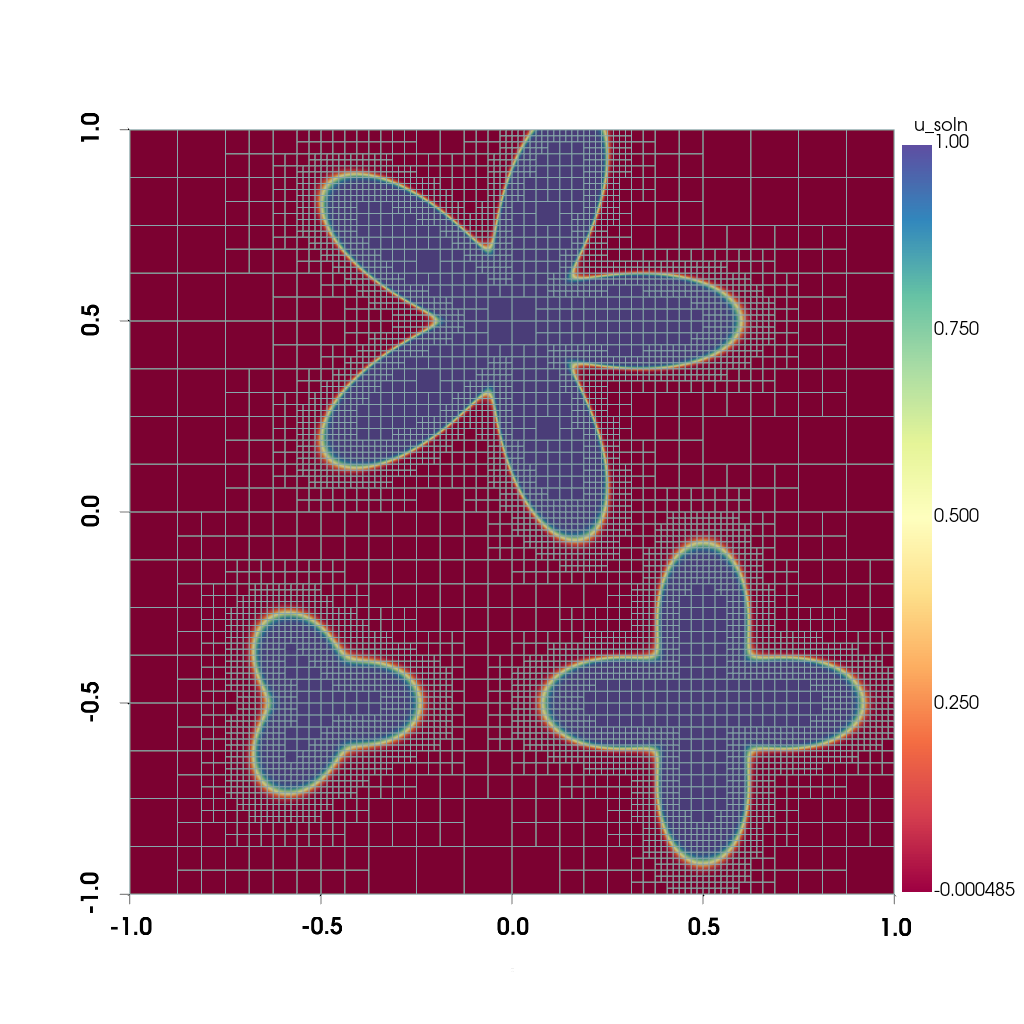
\includegraphics[width=0.75\textwidth, trim={0 100 0 0}]{figures/plot_polar_star.png}
    \caption{The computed solution and mesh for the polar star Poisson problem (\refsec{sub:example-two}). Each patch has a $16 \times 16$ cell-centered grid. The mesh is refined according to the right-hand side and is refined with 8 levels of refinement.}
    \label{fig:polar_star_plot}
\end{figure}

\begin{table}
    \caption{Convergence analysis for the polar star Poisson problem (\refsec{sub:example-two}). The upper part shows convergence for a uniformly refined mesh, while the lower part shows convergence for an adaptively refined mesh. $M$ is the size of the grid on each leaf patch, $L_{\text{max}}$ is the maximum level of refinement, $R_{\text{eff}}$ is the effective resolution for a uniformly refined mesh, DOFs is the total degrees of freedom (i.e., total mesh points), $L_{\infty}$ error is the infinity norm error, $L_{\infty}$ order is the infinity norm convergence order, $L_1$ error is the $1^{\text{st}}$ norm error, and $L_1$ order is the $1^{\text{st}}$ norm convergence order.}
    \centering
    \sisetup{
        table-alignment-mode=format
    }
    \begin{tabular}{
        |
        S   % Patch size
        S[table-column-width=0.8cm]   % Max level
        S[table-text-alignment=right, table-column-width=0.7cm]   % Effective resolution
        S[table-text-alignment=right, table-column-width=1.4cm]   % DOFs
        S[scientific-notation=true, round-mode=places, round-precision=2, table-column-width=1.65cm]   % L-inf error
        S[scientific-notation=false, exponent-mode=fixed, round-mode=places, round-precision=2, table-column-width=1.5cm]   % L-inf order
        S[scientific-notation=true, round-mode=places, round-precision=2]   % L-1 error
        S[scientific-notation=false, exponent-mode=fixed, round-mode=places, round-precision=2]   % L-1 order
        |
    }
\hline
{M} & {$L_{\text{max}}$} & {$R_{\text{eff}}$} & {DOFs} & {$L_{\infty}$ Error} & {$L_{\infty}$ Order} & {$L_1$ Error} & {$L_1$ Order} \\
\hline
\num{16} & \num{4} & \num{256} & \num{65536} & \num{1.56199870806249E+00} & \num{3.03980331387296E+00} & \num{1.65069071070283E-01} & \num{4.25135175327624E+00} \\
\num{16} & \num{5} & \num{512} & \num{262144} & \num{2.79704505790678E-02} & \num{5.80334595545976E+00} & \num{9.84718059820731E-04} & \num{7.38914339546720E+00} \\
\num{16} & \num{6} & \num{1024} & \num{1048576} & \num{5.25422685067089E-03} & \num{2.41235309940473E+00} & \num{7.39997994016763E-05} & \num{3.73411745253242E+00} \\
\num{16} & \num{7} & \num{2048} & \num{4194304} & \num{1.28369442835374E-03} & \num{2.03317666696840E+00} & \num{1.84035492646184E-05} & \num{2.00753733205534E+00} \\
\num{32} & \num{3} & \num{256} & \num{65536} & \num{1.56199870806260E+00} & \num{3.03980331387287E+00} & \num{1.65069071070315E-01} & \num{4.25135175327601E+00} \\
\num{32} & \num{4} & \num{512} & \num{262144} & \num{2.79704505792760E-02} & \num{5.80334595544912E+00} & \num{9.84718059909330E-04} & \num{7.38914339533767E+00} \\
\num{32} & \num{5} & \num{1024} & \num{1048576} & \num{5.25422685134335E-03} & \num{2.41235309923083E+00} & \num{7.39997994074657E-05} & \num{3.73411745254936E+00} \\
\num{32} & \num{6} & \num{2048} & \num{4194304} & \num{1.28369443102049E-03} & \num{2.03317666415598E+00} & \num{1.84035493232030E-05} & \num{2.00753732757563E+00} \\
\hline
\num{16} & \num{4} & \num{256} & \num{50944} & \num{1.56155552227466E+00} & \num{3.04021270772076E+00} & \num{1.64990394749018E-01} & \num{4.25203954412867E+00} \\
\num{16} & \num{5} & \num{512} & \num{171520} & \num{7.12119724134531E-02} & \num{4.45472024347345E+00} & \num{1.03166637134095E-03} & \num{7.32126173153682E+00} \\
\num{16} & \num{6} & \num{1024} & \num{476416} & \num{9.14563250417531E-02} & \num{-3.60963136314842E-01} & \num{1.78815639727227E-04} & \num{2.52843166634489E+00} \\
\num{16} & \num{7} & \num{2048} & \num{1587712} & \num{2.81786611011458E-02} & \num{1.69847988484306E+00} & \num{6.32775510074655E-05} & \num{1.49870725401785E+00} \\
\num{32} & \num{3} & \num{256} & \num{65536} & \num{1.56199870806260E+00} & \num{3.03980331387287E+00} & \num{1.65069071070315E-01} & \num{4.25135175327601E+00} \\
\num{32} & \num{4} & \num{512} & \num{203776} & \num{2.79706867876203E-02} & \num{5.80333377204982E+00} & \num{9.84314973348746E-04} & \num{7.38973407206102E+00} \\
\num{32} & \num{5} & \num{1024} & \num{701440} & \num{2.33901397925928E-02} & \num{2.58015193873839E-01} & \num{8.15186205620300E-05} & \num{3.59391849705353E+00} \\
\num{32} & \num{6} & \num{2048} & \num{1921024} & \num{2.81786212280739E-02} & \num{-2.68700538645513E-01} & \num{3.10231851870699E-05} & \num{1.39378282159843E+00} \\
\hline
    \end{tabular}
    \label{tab:polar_star_results}
\end{table}

\begin{table}
    \caption{Timing and memory results for the Polar Star Poisson problem (\refsec{sub:example-two}). The upper part shows results for the uniformly refined mesh, while the lower part shows results for the adaptively refined mesh. The results here are for a patch size of $16 \times 16$. $L_{\text{max}}$ is the maximum level of refinement, $R_{\text{eff}}$ is the effective resolution, DOFs is the total degrees of freedom, $T_{\text{build}}$ is the time in seconds for the build stage, $T_{\text{upwards}}$ is the time in seconds for the upwards stage, $T_{\text{solve}}$ is the time in seconds for the solve stage, and $S$ is the memory storage in megabytes to store the quadtree and all data matrices stored in each node of the quadtree.}
    \centering
    \sisetup{
        table-alignment-mode=format
    }
    \begin{tabular}{
        |
        S[table-column-width=0.8cm]   % Max level
        S[table-text-alignment=right, table-column-width=0.7cm]   % Effective resolution
        S[table-text-alignment=right, table-column-width=1.4cm]   % DOFs
        S[table-text-alignment=right, scientific-notation=false, exponent-mode=fixed, round-mode=places, round-precision=2]   % Build time
        S[table-text-alignment=right, scientific-notation=false, exponent-mode=fixed, round-mode=places, round-precision=2]   % Upwards time
        S[table-text-alignment=right, scientific-notation=false, exponent-mode=fixed, round-mode=places, round-precision=2]   % Solve time
        S[table-text-alignment=right, scientific-notation=false, exponent-mode=fixed, round-mode=places, round-precision=2]   % Memory size
        |
    }
\hline
{$L_{\text{max}}$} & {$R_{\text{eff}}$} & {DOFs} & {$T_{\text{build}}$ (sec)} & {$T_{\text{upwards}}$ (sec)} & {$T_{\text{solve}}$ (sec)} & {$S$ (MB)} \\
\hline
\num{4} & \num{256} & \num{65536} & \num{1.60620216600000E+00} & \num{4.159940420000E-01} & \num{2.08710665999999E-01} & \num{8.15484972000122E+01} \\
\num{5} & \num{512} & \num{262144} & \num{7.76756095899999E+00} & \num{1.969481791000E+00} & \num{9.65551166999999E-01} & \num{3.98233067512512E+02} \\
\num{6} & \num{1024} & \num{1048576} & \num{3.56706281669999E+01} & \num{9.239545625000E+00} & \num{4.09653733299999E+00} & \num{1.88101041126251E+03} \\
\num{7} & \num{2048} & \num{4194304} & \num{1.65943133041000E+02} & \num{4.246258775000E+01} & \num{1.93515662920000E+01} & \num{8.67619791126251E+03} \\
\hline
\num{4} & \num{256} & \num{50944} & \num{9.29590041999999E-01} & \num{2.385920420000E-01} & \num{8.11892919999999E-02} & \num{3.35243158340454E+01} \\
\num{5} & \num{512} & \num{171520} & \num{3.32502091600000E+00} & \num{7.851652910000E-01} & \num{1.44476500000000E-01} & \num{1.15864575386047E+02} \\
\num{6} & \num{1024} & \num{476416} & \num{9.06574687500000E+00} & \num{1.937123083000E+00} & \num{3.00085959000000E-01} & \num{2.95106141090393E+02} \\
\num{7} & \num{2048} & \num{1587712} & \num{3.07760261670000E+01} & \num{7.226564708000E+00} & \num{1.12108816699999E+00} & \num{1.07681472492218E+03} \\
\hline
    \end{tabular}
    \label{tab:polar_star_timing}
\end{table}

{\bf Results and Discussion}
The polar star Poisson problem is able to highlight the benefits of an adaptive mesh. As shown in \reffig{fig:polar_star_plot}, there is room for significant speed up on the areas outside each polar star. The localized curvature is sufficiently captured by this adaptive scheme. \reftab{tab:polar_star_results} show the error analysis for this problem. Because of the large curvature at the boundaries of a polar star and our use of a second-order accurate solver, the $L_{\infty}$ error is larger than the first Poisson equation from \refsec{sub:example_one}, but we can still achieve 6 digits of accuracy in the $L_1$ norm. The timing results shown in \reftab{tab:polar_star_timing} show significant speed up between the uniform and adaptive implementations. The build time has a $5.5$ times speed up, the upwards stage has a $5.8$ times speed up, and the solve stage has a $17$ times speed up. Plus, the memory for the adaptive case is about $1/8th$ of the memory required for the uniform case.

\subsection{A Helmholtz Equation}
\label{sub:example-three}

We now seek to solve the boundary value problem
\begin{align}
    \nabla^2 u(x,y) + \lambda u(x,y) = f(x,y),
\end{align}
on the square domain $\Omega = [-0.5, 0.5] \times [-0.5, 0.5]$ and subject to Dirichlet boundary conditions which are supplied via the exact solution discussed below.

To provide an analytical solution to compare against, we use a problem provided in \citep{cheng2006adaptive} where they solve Helmholtz's equation on an adaptive mesh. The manufactured solution is
\begin{align}
    u(\textbf{x}) = \sum_{i=1}^{3} e^{-\alpha |\textbf{x} - \textbf{x}_i|^2}
\end{align}
with $\lambda=0.01$, $\alpha=50$, $\textbf{x}_1 = (0.1, 0.1)$, $\textbf{x}_2 = (0, 0)$, and $\textbf{x}_3 = (-0.15, 0.1)$. The right-hand side is computed analytical via the Mathematica software \citep{wolfram2023mathematica} and is used as the refinement criteria. We set the threshold for refinement to $60$. The solution and right-hand side function for $16 \times 16$ patches are plotted in \reffig{fig:helmholtz_u_plot} and \reffig{fig:helmholtz_f_plot}.

{\bf Results and Discussion}
As demonstrated with this example, the implemented \gls{qahps} method solves Helmholtz equations as well with the expected second order accuracy. See \reftab{tab:helmholtz_results} for error and convergence analysis. The adaptive mesh is able to successfully capture the curvature and reduce the work required to solve this equation. \reftab{tab:helmholtz_timing} show timing and memory usage results, which show significant speedup due to good mesh adaptation. We achieve a $17$ times speedup for the build and upwards stage and a $57$ times speedup for the solve stage. Memory is also impressive for this particular problem, with solving the same problem with similar error with $4.6\%$ of the required memory.

\begin{figure}
    \centering
    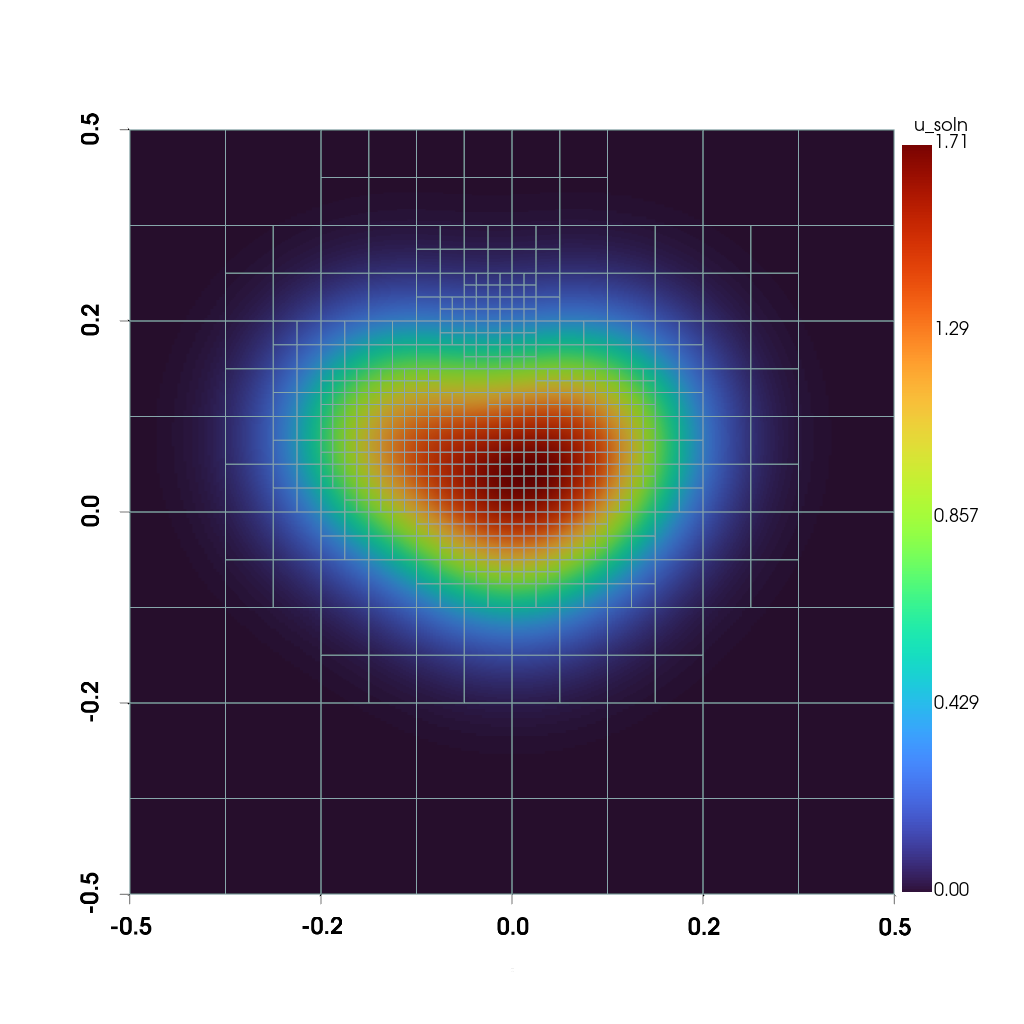
\includegraphics[width=0.75\textwidth, trim={0 100 0 0}]{figures/plot_helmholtz_u.png}
    \caption{Mesh and plot of the solution to the Helmholtz problem in \refsec{sub:example-three}.}
    \label{fig:helmholtz_u_plot}
\end{figure}

\begin{figure}
    \centering
    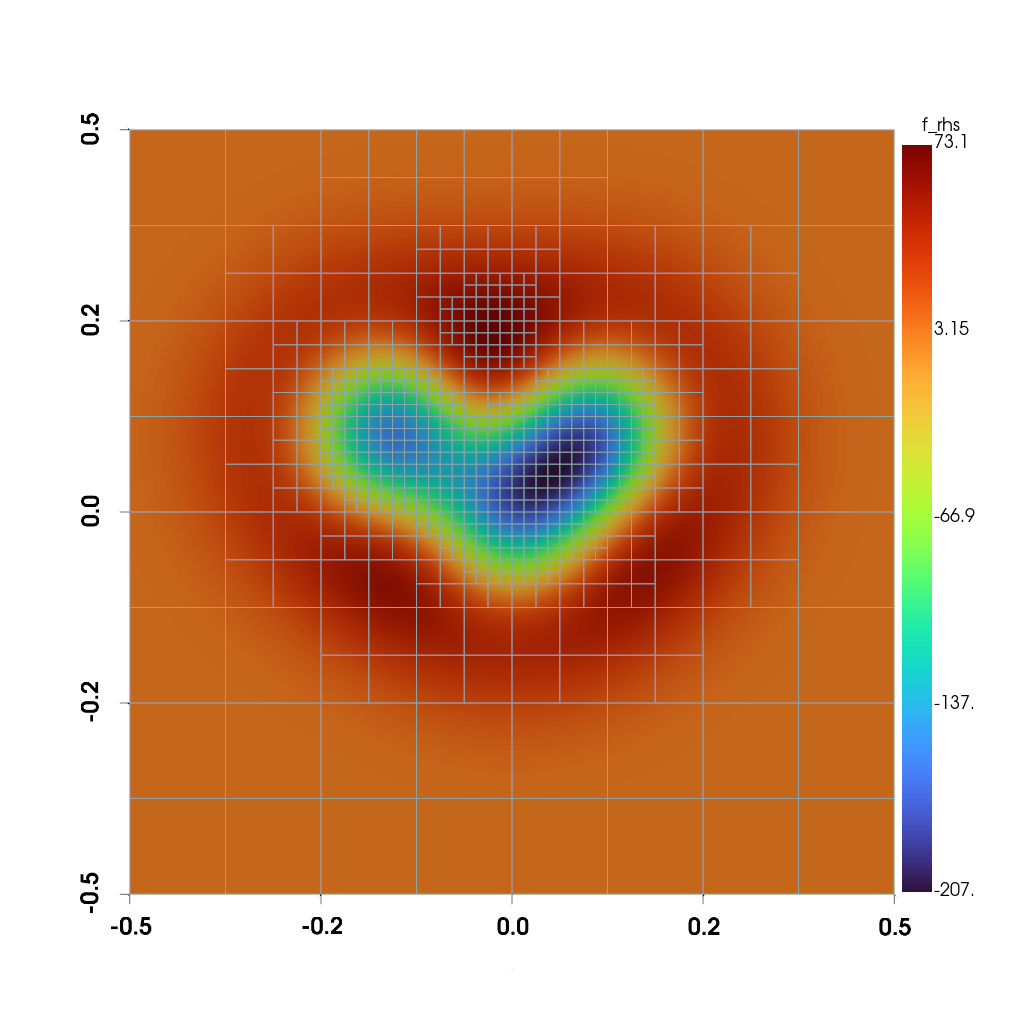
\includegraphics[width=0.75\textwidth, trim={0 100 0 0}]{figures/plot_helmholtz_f.png}
    \caption{Mesh and right-hand side of the solution to the Helmholtz problem in \refsec{sub:example-three}.}
    \label{fig:helmholtz_f_plot}
\end{figure}

\begin{table}
    \caption{Convergence analysis for the Helmholtz problem (\refsec{sub:example-three}). The upper part shows convergence for a uniformly refined mesh, while the lower part shows convergence for an adaptively refined mesh. $M$ is the size of the grid on each leaf patch, $L_{\text{max}}$ is the maximum level of refinement, $R_{\text{eff}}$ is the effective resolution for a uniformly refined mesh, DOFs is the total degrees of freedom (i.e., total mesh points), $L_{\infty}$ error is the infinity norm error, $L_{\infty}$ order is the infinity norm convergence order, $L_1$ error is the $1^{\text{st}}$ norm error, and $L_1$ order is the $1^{\text{st}}$ norm convergence order.}
    \centering
    \sisetup{
        table-alignment-mode=format
    }
    \begin{tabular}{
        |
        S   % Patch size
        S[table-column-width=0.8cm]   % Max level
        S[table-text-alignment=right, table-column-width=0.7cm]   % Effective resolution
        S[table-text-alignment=right, table-column-width=1.4cm]   % DOFs
        S[scientific-notation=true, round-mode=places, round-precision=2, table-column-width=1.65cm]   % L-inf error
        S[scientific-notation=false, exponent-mode=fixed, round-mode=places, round-precision=2, table-column-width=1.5cm]   % L-inf order
        S[scientific-notation=true, round-mode=places, round-precision=2]   % L-1 error
        S[scientific-notation=false, exponent-mode=fixed, round-mode=places, round-precision=2]   % L-1 order
        |
    }
\hline
{M} & {$L_{\text{max}}$} & {$R_{\text{eff}}$} & {DOFs} & {$L_{\infty}$ Error} & {$L_{\infty}$ Order} & {$L_1$ Error} & {$L_1$ Order} \\
\hline
% \num{16} & \num{1} & \num{32} & \num{1024} & \num{1.29237401760500E-02} & \num{0.00000000000000E+00} & \num{1.41621768661641E-03} & \num{0.00000000000000E+00} \\
% \num{16} & \num{2} & \num{64} & \num{4096} & \num{3.24474376001426E-03} & \num{1.99384719443466E+00} & \num{3.52042103641637E-04} & \num{2.00822315072563E+00} \\
\num{16} & \num{3} & \num{128} & \num{16384} & \num{8.11856103331010E-04} & \num{1.99880860589163E+00} & \num{8.79086298739653E-05} & \num{2.00167127817603E+00} \\
\num{16} & \num{4} & \num{256} & \num{65536} & \num{2.02984786720650E-04} & \num{1.99985243641999E+00} & \num{2.19695214703194E-05} & \num{2.00050135378016E+00} \\
\num{16} & \num{5} & \num{512} & \num{262144} & \num{5.07454266427398E-05} & \num{2.00002189203670E+00} & \num{5.49192113777069E-06} & \num{2.00012063189787E+00} \\
\num{16} & \num{6} & \num{1024} & \num{1048576} & \num{1.26864921798919E-05} & \num{1.99998458881074E+00} & \num{1.37295318659519E-06} & \num{2.00002847405489E+00} \\
\num{16} & \num{7} & \num{2048} & \num{4194304} & \num{3.17161259033582E-06} & \num{2.00000475557083E+00} & \num{3.43237939677034E-07} & \num{2.00000150042016E+00} \\
% \num{32} & \num{1} & \num{64} & \num{4096} & \num{3.24474376001093E-03} & \num{0.00000000000000E+00} & \num{3.52042103642942E-04} & \num{0.00000000000000E+00} \\
% \num{32} & \num{2} & \num{128} & \num{16384} & \num{8.11856103339447E-04} & \num{1.99880860587515E+00} & \num{8.79086298732444E-05} & \num{2.00167127819321E+00} \\
\num{32} & \num{3} & \num{256} & \num{65536} & \num{2.02984786837223E-04} & \num{1.99985243560645E+00} & \num{2.19695214601884E-05} & \num{2.00050135443361E+00} \\
\num{32} & \num{4} & \num{512} & \num{262144} & \num{5.07454269149665E-05} & \num{2.00002188512581E+00} & \num{5.49192111200352E-06} & \num{2.00012063800147E+00} \\
\num{32} & \num{5} & \num{1024} & \num{1048576} & \num{1.26864947160854E-05} & \num{1.99998430813683E+00} & \num{1.37295295907976E-06} & \num{2.00002870635855E+00} \\
\num{32} & \num{6} & \num{2048} & \num{4194304} & \num{3.17160773866120E-06} & \num{2.00000725090321E+00} & \num{3.43238375314458E-07} & \num{1.99999943028095E+00} \\
\hline
% \num{16} & \num{1} & \num{32} & \num{1024} & \num{1.29237401760500E-02} & \num{0.00000000000000E+00} & \num{1.41621768661641E-03} & \num{0.00000000000000E+00} \\
% \num{16} & \num{2} & \num{64} & \num{4096} & \num{3.24474376001426E-03} & \num{1.99384719443466E+00} & \num{3.52042103641637E-04} & \num{2.00822315072563E+00} \\
\num{16} & \num{3} & \num{128} & \num{8704} & \num{1.35786298229745E-03} & \num{1.25676664286521E+00} & \num{1.62110560935590E-04} & \num{1.11876990262527E+00} \\
\num{16} & \num{4} & \num{256} & \num{22528} & \num{1.64905762929112E-03} & \num{-2.80303908147837E-01} & \num{8.45781698947318E-05} & \num{9.38620831715358E-01} \\
\num{16} & \num{5} & \num{512} & \num{54784} & \num{2.38573635354355E-03} & \num{-5.32792803144748E-01} & \num{3.38667165953099E-05} & \num{1.32041722042279E+00} \\
\num{16} & \num{6} & \num{1024} & \num{163072} & \num{5.94628321314072E-04} & \num{2.00437453684095E+00} & \num{1.31283531083692E-05} & \num{1.36718217508683E+00} \\
\num{16} & \num{7} & \num{2048} & \num{485632} & \num{7.32427776781507E-04} & \num{-3.00698326888675E-01} & \num{1.91363184831188E-05} & \num{-5.43627357312482E-01} \\
% \num{32} & \num{1} & \num{64} & \num{4096} & \num{3.24474376001093E-03} & \num{0.00000000000000E+00} & \num{3.52042103642942E-04} & \num{0.00000000000000E+00} \\
% \num{32} & \num{2} & \num{128} & \num{16384} & \num{8.11856103339447E-04} & \num{1.99880860587515E+00} & \num{8.79086298732444E-05} & \num{2.00167127819321E+00} \\
\num{32} & \num{3} & \num{256} & \num{34816} & \num{3.39042440507864E-04} & \num{1.25975816324197E+00} & \num{4.06849021440135E-05} & \num{1.11151127906479E+00} \\
\num{32} & \num{4} & \num{512} & \num{90112} & \num{4.02109898754332E-04} & \num{-2.46123973731869E-01} & \num{2.13036585418219E-05} & \num{9.33392310591107E-01} \\
\num{32} & \num{5} & \num{1024} & \num{222208} & \num{5.85657916098325E-04} & \num{-5.42468378289773E-01} & \num{8.31054203108411E-06} & \num{1.35808672932660E+00} \\
\num{32} & \num{6} & \num{2048} & \num{664576} & \num{1.50576960741055E-04} & \num{1.95955718461569E+00} & \num{3.71801364039699E-06} & \num{1.16041051254945E+00} \\
\hline
    \end{tabular}
    \label{tab:helmholtz_results}
\end{table}

\begin{table}
    \caption{Timing and memory results for the Helmholtz problem (\refsec{sub:example-three}). The upper part shows results for the uniformly refined mesh, while the lower part shows results for the adaptively refined mesh. The results here are for a patch size of $16 \times 16$. $L_{\text{max}}$ is the maximum level of refinement, $R_{\text{eff}}$ is the effective resolution, DOFs is the total degrees of freedom, $T_{\text{build}}$ is the time in seconds for the build stage, $T_{\text{upwards}}$ is the time in seconds for the upwards stage, $T_{\text{solve}}$ is the time in seconds for the solve stage, and $S$ is the memory storage in megabytes to store the quadtree and all data matrices stored in each node of the quadtree.}
    \centering
    \sisetup{
        table-alignment-mode=format
    }
    \begin{tabular}{
        |
        S[table-column-width=0.8cm]   % Max level
        S[table-text-alignment=right, table-column-width=0.7cm]   % Effective resolution
        S[table-text-alignment=right, table-column-width=1.4cm]   % DOFs
        S[table-text-alignment=right, scientific-notation=false, exponent-mode=fixed, round-mode=places, round-precision=2]   % Build time
        S[table-text-alignment=right, scientific-notation=false, exponent-mode=fixed, round-mode=places, round-precision=2]   % Upwards time
        S[table-text-alignment=right, scientific-notation=false, exponent-mode=fixed, round-mode=places, round-precision=2]   % Solve time
        S[table-text-alignment=right, scientific-notation=false, exponent-mode=fixed, round-mode=places, round-precision=2]   % Memory size
        |
    }
\hline
{$L_{\text{max}}$} & {$R_{\text{eff}}$} & {DOFs} & {$T_{\text{build}}$ (sec)} & {$T_{\text{upwards}}$ (sec)} & {$T_{\text{solve}}$ (sec)} & {$S$ (MB)} \\
\hline
\num{3} & \num{128} & \num{16384} & \num{3.01504249999999E-01} & \num{7.933354200E-02} & \num{4.67959999999999E-02} & \num{1.58822374343872E+01} \\
\num{4} & \num{256} & \num{65536} & \num{1.49072670900000E+00} & \num{3.993616660E-01} & \num{1.95166584000000E-01} & \num{8.15484972000122E+01} \\
\num{5} & \num{512} & \num{262144} & \num{7.21594766700000E+00} & \num{1.882675541E+00} & \num{9.14324582999999E-01} & \num{3.98233067512512E+02} \\
\num{6} & \num{1024} & \num{1048576} & \num{3.38984894589999E+01} & \num{8.795803542E+00} & \num{3.89846425000000E+00} & \num{1.88101041126251E+03} \\
\num{7} & \num{2048} & \num{4194304} & \num{1.59021219833999E+02} & \num{4.257397542E+01} & \num{1.88671120829999E+01} & \num{8.67619791126251E+03} \\
\hline
\num{3} & \num{128} & \num{8704} & \num{1.29889625000000E-01} & \num{2.823758300E-02} & \num{1.49769169999999E-02} & \num{4.63061237335205E+00} \\
\num{4} & \num{256} & \num{22528} & \num{3.62822042000000E-01} & \num{8.477891600E-02} & \num{2.33342910000000E-02} & \num{1.33817796707153E+01} \\
\num{5} & \num{512} & \num{54784} & \num{8.70019541999999E-01} & \num{1.982561250E-01} & \num{4.41358329999999E-02} & \num{2.84357728958129E+01} \\
\num{6} & \num{1024} & \num{163072} & \num{2.88925454100000E+00} & \num{7.241970830E-01} & \num{1.29217458000000E-01} & \num{1.16809662818908E+02} \\
\num{7} & \num{2048} & \num{485632} & \num{9.30737075000000E+00} & \num{2.389094875E+00} & \num{3.30502583999999E-01} & \num{3.95934556007385E+02} \\
\hline
    \end{tabular}
    \label{tab:helmholtz_timing}
\end{table}